\documentclass{beamer}

\usetheme{Berlin}
\usecolortheme{Orchid}
\useoutertheme{miniframes}
\setbeamertemplate{navigation symbols}{}

\usepackage[utf8]{inputenc}
\usepackage[T1]{fontenc}
\usepackage{amsmath}
\usepackage{amssymb}
\usepackage{booktabs}
\usepackage{graphicx}
\graphicspath{{../images/}}

\usepackage{xcolor}
\usepackage{listings}
\usepackage{hyperref}
\usepackage{tikz}
\usetikzlibrary{arrows.meta,positioning,shapes.geometric,calc}

\lstset{
  language=Java,
  basicstyle=\ttfamily\small,
  keywordstyle=\color{blue},
  commentstyle=\color{gray},
  stringstyle=\color{teal},
  showstringspaces=false,
  columns=fullflexible,
  breaklines=true
}

% Per-slide source line (references shown on the slide itself).
\newcommand{\slidesources}[1]{%
  \vfill
  {\tiny\color{gray}\raggedright\sloppy\parbox{\linewidth}{Sources: #1}\par}%
}

% Unit-wise source strings for this subject (used by slides/notes).
% Path is relative to the lecture `latex/` folder (the compilation CWD).
% OOPS with Java (CSEG1044) — unit-wise sources
%
% These are short, student-facing reference strings intended to be used with:
%   - \slidesources{...}  (in beamer slides)
%   - \notesources{...}   (in lecture notes)
%
% Style inspiration: other subjects in My-Subjects/ use semicolon-separated sources
% and include an "accessed" date for web documentation.

\newcommand{\OOPSUnitISources}{Schildt, \textit{Java: A Beginner's Guide} (10e), McGraw-Hill (Java fundamentals + OOP basics).; Oracle Java Tutorials: Getting Started + Language Basics + Classes and Objects (accessed \today).; Java SE API docs (e.g., \texttt{String}, \texttt{Scanner}) (accessed \today).}

\newcommand{\OOPSUnitIISources}{Schildt, \textit{Java: The Complete Reference} (12e), McGraw-Hill (classes, inheritance, packages, interfaces).; Bloch, \textit{Effective Java} (3e), Addison-Wesley, 2018 (design choices; interfaces vs abstract classes).; Oracle Java Tutorials: Classes and Objects + Interfaces + Packages (accessed \today).; Java SE API docs (e.g., \texttt{Comparable}, \texttt{Runnable}) (accessed \today).}

\newcommand{\OOPSUnitIIISources}{Schildt, \textit{Java: The Complete Reference} (12e) (nested/inner classes, exceptions, threads, I/O).; Oracle Java Tutorials: Nested Classes + Exceptions + Concurrency + Basic I/O (accessed \today).; Java SE API docs (e.g., \texttt{Thread}, \texttt{AutoCloseable}) (accessed \today).}

\newcommand{\OOPSUnitIVSources}{Schildt, \textit{Java: The Complete Reference} (12e) (generics, lambdas, Swing, JDBC).; Bloch, \textit{Effective Java} (3e) (generics + lambdas).; Oracle Java Tutorials: Generics + Lambda Expressions + Swing + JDBC Basics (accessed \today).; Java SE API docs (e.g., \texttt{java.util.function}, \texttt{javax.swing}, \texttt{java.sql}) (accessed \today).}

\newcommand{\OOPSUnitVSources}{Schildt, \textit{Java: The Complete Reference} (12e) (Collections Framework + wrapper classes).; Oracle Java docs: Collections Framework overview (accessed \today).; Java SE API docs (\texttt{java.util} collections; wrapper classes in \texttt{java.lang}) (accessed \today).}

\newcommand{\OOPSUnitVISources}{Git SCM: \textit{Pro Git} (2e) (version control workflow), accessed \today.; GitHub Docs (repositories, issues, pull requests), accessed \today.; Oracle Java Tutorials: Swing + JDBC (accessed \today).; JUnit 5 User Guide (accessed \today).; Apache Maven Project: Getting Started (accessed \today).; Gradle User Manual: Getting Started (accessed \today).; UML class diagrams: UML 2.x overview/spec (accessed \today).}

\newcommand{\OOPSMiscWhyInterfacesSources}{Schildt, \textit{Java: The Complete Reference} (12e) (interfaces).; Bloch, \textit{Effective Java} (3e) (prefer interfaces where appropriate).; Oracle Java Tutorials: Interfaces (accessed \today).; Java SE API docs (e.g., \texttt{Comparable}, \texttt{Runnable}) (accessed \today).}



\title[OOPS with Java]{Object Oriented Programming (CSEG1044)}
\subtitle{Unit 01 -- Lecture 02: Java Overview + Program Structure + Features}
\begin{document}

\begin{frame}[fragile]
  \titlepage
  \vspace{0.5em}
  \slidesources{\OOPSUnitISources}
\end{frame}

\begin{frame}{Quick Links}
  \centering
  \hyperlink{sec:overview}{\beamerbutton{Overview}}\hspace{0.6em}
  \hyperlink{sec:concepts}{\beamerbutton{Key Topics}}\hspace{0.6em}
  \hyperlink{sec:demo}{\beamerbutton{Demo}}\hspace{0.6em}
  \hyperlink{sec:summary}{\beamerbutton{Summary}}
  \slidesources{\OOPSUnitISources}
\end{frame}

\begin{frame}{Agenda}
  \tableofcontents
  \slidesources{\OOPSUnitISources}
\end{frame}

\section{Overview}
\label{sec:overview}

\begin{frame}{Lecture Snapshot}
\begin{itemize}[<+->]
  \item \textbf{Unit focus:} Introduction to OOPs and Java Fundamentals
  \item \textbf{Course thread:} Use Java Overview + Program Structure + Features to make the first text-based version of Campus Resource Manager easier to reason about before the full object model arrives.
\end{itemize}
  \slidesources{\OOPSUnitISources}
\end{frame}

\begin{frame}{Recall Before You Start}
\begin{itemize}[<+->]
  \item \textbf{OOP vocabulary}: The previous lecture introduced objects, classes, and modelling; this lecture connects them to the Java platform. Main reference: \texttt{Unit 01 / Lecture 01 slides/notes}.
  \item \textbf{Problem to program flow}: Once the model is clear, the next question is how Java compiles and runs it. Main reference: \texttt{Unit 01 / Lecture 01 slides/notes}.
\end{itemize}
  \slidesources{\OOPSUnitISources}
\end{frame}


\begin{frame}{Learning Outcomes}
  \begin{itemize}[<+->]
    \item Explain JDK vs JRE vs JVM and what bytecode is.
    \item Compile and run a Java program; recognize compile-time vs runtime errors.
    \item List key features of Java and their practical meaning.
  \end{itemize}
  \slidesources{\OOPSUnitISources}
\end{frame}

\begin{frame}{Key Terms to Know}
\small
\begin{columns}[t]
\column{0.48\textwidth}
\begin{itemize}
  \item \textbf{JDK (Java Development Kit)}: tools for development (compiler \texttt{javac}, docs, etc.).
  \item \textbf{JRE (Java Runtime Environment)}: runtime needed to run Java apps (JVM + libraries).
  \item \textbf{JVM (Java Virtual Machine)}: executes Java bytecode (\texttt{.class}).
  \item \textbf{Bytecode}: platform-neutral instructions produced by \texttt{javac}.
\end{itemize}
\column{0.48\textwidth}
\begin{itemize}
  \item \textbf{Classpath}: where the JVM looks for compiled classes and libraries.
  \item \textbf{Compile-time error}: detected by the compiler before running.
  \item \textbf{Runtime error/exception}: occurs while the program is executing.
\end{itemize}
\end{columns}
  \slidesources{\OOPSUnitISources}
\end{frame}

\begin{frame}{Study Flow for This Lecture}
\begin{enumerate}[<+->]
  \item Refresh the prerequisite bridge before reading new ideas in isolation.
  \item Study the main build in this order: \textit{Java ecosystem: JDK vs JRE vs JVM} $\rightarrow$ \textit{Bytecode and the compile/run flow} $\rightarrow$ \textit{Basic program structure: class + \texttt{main}} $\rightarrow$ \textit{Compile-time vs runtime errors}.
  \item Trace the worked example and connect each line back to one concept frame.
  \item Attempt the mini exercises before moving to the recap and exit check.
\end{enumerate}
  \slidesources{\OOPSUnitISources}
\end{frame}


\section{Key Topics}
\label{sec:concepts}

\begin{frame}{Unit 01: Introduction to OOPs}
  \begin{itemize}[<+->]
    \item Lecture focus: Java Overview + Program Structure + Features
  \end{itemize}
  \slidesources{\OOPSUnitISources}
\end{frame}

\begin{frame}{Today: Roadmap}
  \begin{itemize}[<+->]
    \item Java ecosystem: JDK/JRE/JVM, bytecode, compile/run flow
    \item Basic program structure: class, `main`, compilation errors vs runtime errors
    \item Features of Java (platform independence, security, GC overview)
  \end{itemize}
  \slidesources{\OOPSUnitISources}
\end{frame}

\begin{frame}{JDK vs JRE vs JVM (picture)}
  \centering
  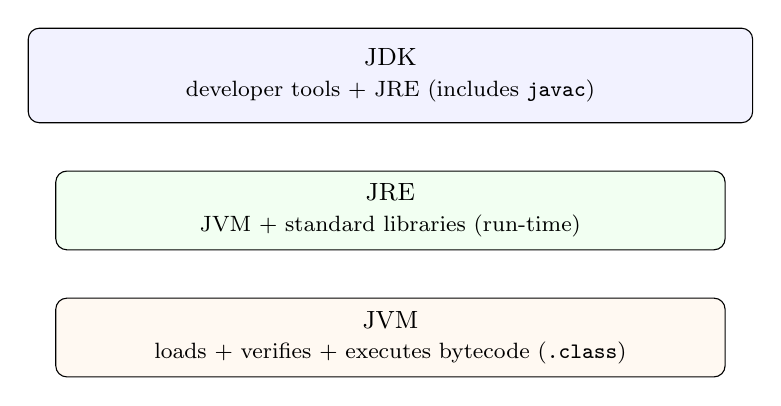
\begin{tikzpicture}[
    box/.style={draw, rounded corners, align=center, minimum width=9.2cm, minimum height=1.2cm, font=\small},
    inner/.style={draw, rounded corners, align=center, minimum width=8.5cm, minimum height=1.0cm, font=\small}
  ]
    \node[box, fill=blue!5] (jdk) {JDK\\\footnotesize developer tools + JRE (includes \texttt{javac})};
    \node[inner, fill=green!5, below=0.6cm of jdk] (jre) {JRE\\\footnotesize JVM + standard libraries (run-time)};
    \node[inner, fill=orange!5, below=0.6cm of jre] (jvm) {JVM\\\footnotesize loads + verifies + executes bytecode (\texttt{.class})};
  \end{tikzpicture}
  \slidesources{\OOPSUnitISources}
\end{frame}

\begin{frame}{Compile $\rightarrow$ Run flow}
  \begin{center}
  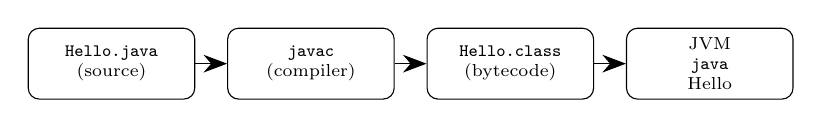
\begin{tikzpicture}[
    node distance=0.45cm,
    every node/.style={transform shape},
    scale=0.9,
    box/.style={draw, rounded corners, align=center, minimum width=2.35cm, minimum height=1.0cm, font=\scriptsize}
  ]
    \node[box] (java) {\texttt{Hello.java}\\(source)};
    \node[box, right=of java] (javac) {\texttt{javac}\\(compiler)};
    \node[box, right=of javac] (class) {\texttt{Hello.class}\\(bytecode)};
    \node[box, right=of class] (jvm) {JVM\\\texttt{java}\\Hello};
    \draw[-{Stealth[length=3mm]}] (java) -- (javac);
    \draw[-{Stealth[length=3mm]}] (javac) -- (class);
    \draw[-{Stealth[length=3mm]}] (class) -- (jvm);
  \end{tikzpicture}
  \end{center}
  \slidesources{\OOPSUnitISources}
\end{frame}

\begin{frame}[fragile]{Program structure (minimum)}
\begin{lstlisting}
public class Hello {
    public static void main(String[] args) {
        System.out.println("Hello, Java!");
    }
}
\end{lstlisting}
  \begin{itemize}[<+->]
    \item If the class is \texttt{public}, file name must be \texttt{Hello.java}.
    \item JVM starts execution from \texttt{main}.
  \end{itemize}
  \slidesources{\OOPSUnitISources}
\end{frame}

\begin{frame}{Compile-time vs Runtime (quick)}
  \begin{itemize}[<+->]
    \item \textbf{Compile-time error:} caught by \texttt{javac} (syntax/type errors).
    \item \textbf{Runtime exception:} program compiles but fails while running.
  \end{itemize}
  \vspace{0.4em}
  \begin{block}{Examples}
    \begin{itemize}
      \item Compile-time: missing semicolon, ``cannot find symbol''
      \item Runtime: \texttt{ArithmeticException}, \texttt{NullPointerException}
    \end{itemize}
  \end{block}
  \slidesources{\OOPSUnitISources}
\end{frame}

\begin{frame}{Features of Java (what you get)}
  \begin{itemize}[<+->]
    \item Platform independent: bytecode + JVM
    \item Strongly typed: many errors caught early
    \item Garbage collection: automatic memory management
    \item Rich libraries: collections, I/O, GUI, DB, networking
    \item Security model: class loading + bytecode verification
  \end{itemize}
  \slidesources{\OOPSUnitISources}
\end{frame}

\begin{frame}{Checkpoint and Reflection}
\begin{block}{Reflection prompt}
Where would \textit{Java Overview + Program Structure + Features} matter most in Campus Resource Manager, and which design choice would you justify using this lecture's ideas?
\end{block}
\begin{block}{Quick self-check}
Which part needs one more example before you move on: \textit{Java ecosystem: JDK vs JRE vs JVM}, \textit{Bytecode and the compile/run flow}, the worked example, or the recap?
\end{block}
  \slidesources{\OOPSUnitISources}
\end{frame}

\section{Demo / Example}
\label{sec:demo}

\begin{frame}[fragile]{Demo: \texttt{javac} and \texttt{java}}
\begin{lstlisting}
public class Hello {
    public static void main(String[] args) {
        System.out.println("Hello, Java!");
    }
}
\end{lstlisting}
  \vspace{0.4em}
  \begin{itemize}[<+->]
    \item Compile: \texttt{javac Hello.java}
    \item Run: \texttt{java Hello}
    \item Try: change message and re-run.
  \end{itemize}
  \slidesources{\OOPSUnitISources}
\end{frame}

\begin{frame}[fragile]{Demo: runtime exception (observe)}
\begin{lstlisting}
public class DivideDemo {
    public static void main(String[] args) {
        int a = 10, b = 0;
        System.out.println(a / b);
    }
}
\end{lstlisting}
  \slidesources{\OOPSUnitISources}
\end{frame}

\begin{frame}{Mini Exercises (2--3 mins)}
  \begin{enumerate}[<+->]
    \item Which contains \texttt{javac}: JDK, JRE, or JVM?
    \item If you write \texttt{public class Student}, what should the file be named?
    \item Is ``cannot find symbol'' compile-time or runtime?
  \end{enumerate}
  \slidesources{\OOPSUnitISources}
\end{frame}

\begin{frame}{Watch-outs}
\begin{itemize}[<+->]
  \item Using JDK, JRE, and JVM as interchangeable terms.
  \item Forgetting that a public class name must match the file name.
  \item Mixing compile-time errors with runtime failures.
\end{itemize}
  \slidesources{\OOPSUnitISources}
\end{frame}

\section{Summary}
\label{sec:summary}

\begin{frame}{Key Takeaways}
  \begin{itemize}[<+->]
    \item JDK is for development (includes \texttt{javac}); JRE/JVM are for running.
    \item Java compiles to bytecode (\texttt{.class}) and runs on the JVM.
    \item Compile-time errors stop compilation; runtime exceptions happen while running.
  \end{itemize}
  \slidesources{\OOPSUnitISources}
\end{frame}

\begin{frame}{Checkpoint Questions}
  \begin{enumerate}[<+->]
    \item Why does Java use bytecode?
    \item Give one compile-time error example and one runtime exception example.
    \item What is the role of \texttt{main}?
  \end{enumerate}
  \slidesources{\OOPSUnitISources}
\end{frame}

\begin{frame}{Next Study Steps}
\begin{itemize}[<+->]
  \item Revisit the recall references if any older idea still feels weak.
  \item Rework the lecture example without looking at the notes first.
  \item Attempt the self-study practice and then answer the exit questions in full sentences.
  \item Apply the idea once inside Campus Resource Manager to make the concept stick.
\end{itemize}
  \slidesources{\OOPSUnitISources}
\end{frame}

\begin{frame}{Next Lecture Preview}
  \textbf{Next:} I/O + Command Line + Types + Operators
  \vspace{0.6em}
  \begin{itemize}[<+->]
    \item Practice running a program with command line arguments.
    \item Revise basic numeric types and operator precedence.
  \end{itemize}
  \slidesources{\OOPSUnitISources}
\end{frame}

\end{document}
